\section{Results}
\label{sec:results}

\subsection{Token Size and Bytes on the Wire}
\label{sec:res-size}

\begin{figure}[t]
\centering
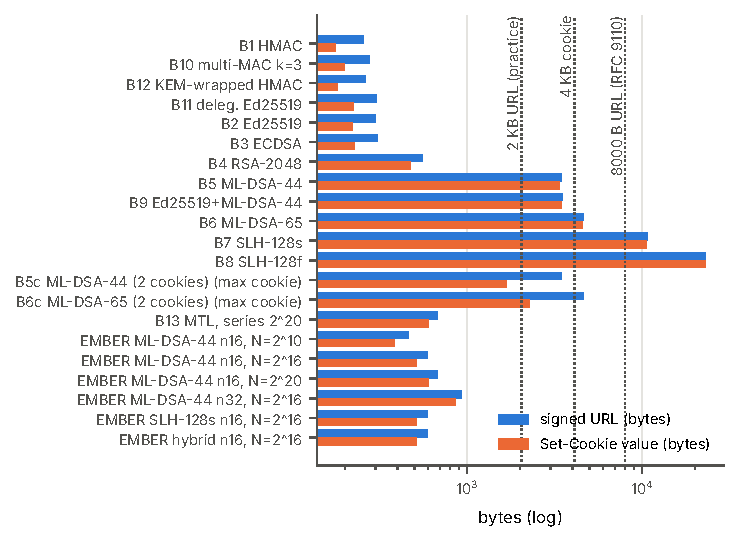
\includegraphics[width=\columnwidth]{figures/fig2_token_sizes.pdf}
\caption{Encoded token size per scheme (measured; 60-character path). Vertical lines: 2~KB URL practice, 4096-B cookie~\cite{rfc6265}, 8000-B URL recommendation~\cite{rfc9110}.}
\label{fig:sizes}
\end{figure}

Fig.~\ref{fig:sizes} shows measured token sizes. Per-token post-quantum signatures do not fit: B5 (ML-DSA-44) is \num{3350}~B, B6 \num{4535}~B, B7 \num{10598}~B and B8 \num{22907}~B, and the B9 hybrid is \num{3435}~B. Under a lognormal URL-path assumption (median 80 characters), no B5 or B6 signed URL fits in 2~KB, no B6 cookie fits in 4096~B, and B7/B8 fit no limit. Classical tokens are 166~B (B1), 209~B (B2) and 465~B (B4). The strong symmetric and delegated baselines are smaller than EMBER: B12 is 171~B, B11 214~B and B10 187~B for $k=3$. EMBER O1 grows by about 21~B per tree level. It is 375~B at $N=2^{10}$, 503~B at $2^{16}$, 588~B at $2^{20}$ and 673~B at $2^{24}$. With $n=32$ (O2) it is 844~B at $2^{16}$. EMBER is therefore 6.7$\times$ smaller than B5 at $N=2^{16}$, but it stays under 512~B only up to $N=2^{16}$, not up to $2^{20}$ as we had hypothesized. The MTL condensed signature (B13) has the same size at the same tree size (504~B for a $2^{16}$ series). The difference is that MTL's series grows with $\lambda\vmax$, whereas EMBER's tree grows only with $\lambda\Delta$. Eq.~\eqref{eq:size} matches all 26 measured EMBER sizes exactly (Fig.~\ref{fig:sizeN}, top).

\begin{table}[t]
\centering
\caption{Upstream request-header bytes per session (1 manifest + 150 segments; measured with Go HPACK, 4096-B table unless noted).}
\label{tab:wire}
\footnotesize
\setlength{\tabcolsep}{3pt}
\begin{tabular}{@{}lrrrr@{}}
\toprule
Scheme, placement & token B & h2 & HTTP/1.1 & h2, 64~KiB \\
\midrule
No token & 0 & \num{8557} & \num{86823} & \num{8761} \\
B1 HMAC, URL & 127 & \num{26706} & \num{107057} & \num{24918} \\
B11 deleg.\ Ed25519, URL & 175 & \num{33277} & \num{114305} & \num{30825} \\
B12 KEM-wrapped, URL & 132 & \num{27660} & \num{107812} & \num{25540} \\
B5 ML-DSA-44, URL & \num{3311} & \num{457831} & \num{587841} & \num{410359} \\
B5 ML-DSA-44, cookie & \num{3311} & \num{458568} & \num{589955} & \num{11667} \\
B5c, 2 cookies & \num{3311} & \num{460984} & \num{592522} & \num{11933} \\
O1 $N{=}2^{14}$, URL & 421 & \num{66344} & \num{151451} & \num{60605} \\
O1 $N{=}2^{14}$, URL + staple & 421 & \num{69298} & \num{154749} & \num{63149} \\
O1 $N{=}2^{14}$, cookie & 421 & \num{10775} & \num{153565} & \num{9358} \\
O1 $N{=}2^{20}$, URL & 549 & \num{83225} & \num{170779} & \num{75820} \\
\bottomrule
\end{tabular}
\end{table}

Fitting a budget is guaranteed by construction (the count trigger), so the more informative metric is bytes per session (Table~\ref{tab:wire}). Token sizes in this experiment are smaller because of its different claim string. In URL form, an EMBER session uses \num{66344}~B under HTTP/2, which is 0.144$\times$ the split-cookie ML-DSA-44 baseline (B5c) and meets our hypothesis of at most 0.25$\times$. Under HTTP/1.1 the ratio is 0.256$\times$ and narrowly misses it, because about 87~KB per session are token-independent headers. In cookie form the outcome depends on the HPACK table size. With the default 4096-B table, the 3.3~KB ML-DSA cookie is evicted by the changing \texttt{:path} entries and is re-sent on every request (\num{3036.9}~B per request), and splitting it into two cookies does not help. With a 64~KiB table the cookie stays indexed, and the gap nearly vanishes: \num{11667}~B for B5 versus \num{9358}~B for EMBER. Stapling the root costs \num{2954}~B once per session under HTTP/2.

\begin{figure}[t]
\centering
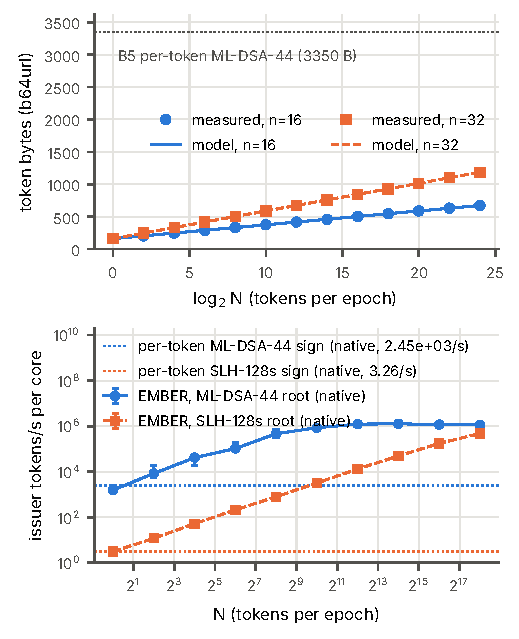
\includegraphics[width=\columnwidth]{figures/fig3_size_vs_N.pdf}
\caption{Top: EMBER token size vs.\ $\log_2 N$ (markers measured, lines Eq.~\eqref{eq:size}). Bottom: native issuer throughput per core (OpenSSL~3.5.4, run~2), with per-token signing rates as horizontal lines.}
\label{fig:sizeN}
\end{figure}

\subsection{Edge Verification Cost}
\label{sec:res-cpu}

\begin{figure*}[t]
\centering
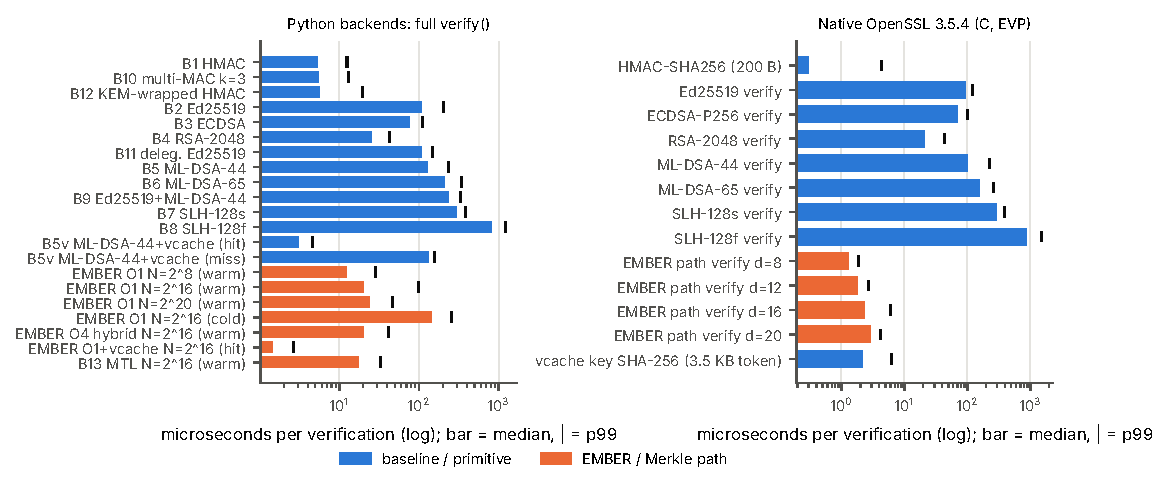
\includegraphics[width=\textwidth]{figures/fig4_verify_cost.pdf}
\caption{Per-verification cost (bar: median; tick: p99). Left: Python reference, full \texttt{verify()} (secondary source). Right: native OpenSSL~3.5.4 primitives and EMBER path verification (primary source, run~2).}
\label{fig:verify}
\end{figure*}

Fig.~\ref{fig:verify} and Table~\ref{tab:primitives} give per-verification costs. Natively, ML-DSA-44 verification takes 100.9\us{} [100.2, 120.4], close to Ed25519 (94.6\us). A warm EMBER path at $d=16$ takes 2.34\us{} [2.33, 2.46]. That is 43$\times$ cheaper than ML-DSA-44 verification, but 7.9$\times$ the 0.30\us{} of HMAC-SHA256 over the 200-B claims. Our hypothesis of at most 5$\times$ HMAC holds only for $d\le8$ (1.28\us, 4.3$\times$). Path cost grows by about 0.13\us{} per level, from 0.75\us{} at $d=4$ to 3.41\us{} at $d=24$. The Go implementation gives a smaller ratio: a full EMBER token verification (parse plus path, $N=2^{14}$) takes 3.074\us, which is 3.6$\times$ Go HMAC verification (0.853\us) and 10.7$\times$ cheaper than circl ML-DSA-44 verification (32.76\us). circl's ML-DSA-44 verification is 3.6--4.0$\times$ faster than OpenSSL's, outside the 3$\times$ cross-implementation bound we set in advance. We attribute this to circl's optimized arithmetic and report it rather than hide it.

\begin{table}[t]
\centering
\caption{Native primitive costs (OpenSSL~3.5.4, run~2; median [95\% CI], \textmu s; sizes in bytes).}
\label{tab:primitives}
\footnotesize
\setlength{\tabcolsep}{1.6pt}
\begin{tabular}{@{}lrrll@{}}
\toprule
Scheme & pk & sig & sign & verify \\
\midrule
HMAC-SHA256 & -- & 32 & 0.30 [0.30, 0.30] & 0.30 [0.30, 0.30] \\
Ed25519 & 32 & 64 & 30.1 [30.1, 30.4] & 94.6 [93.8, 96.2] \\
ECDSA P-256 & 65 & 71 & 23.0 [22.9, 31.1] & 69.6 [69.5, 70.0] \\
RSA-2048 & 270 & 256 & 314.1 [309.4, 340.5] & 20.7 [18.8, 24.2] \\
ML-DSA-44 & 1312 & 2420 & 408.8 [386.9, 452.4] & 100.9 [100.2, 120.4] \\
ML-DSA-65 & 1952 & 3309 & 676.5 [673.5, 682.7] & 154.8 [154.6, 165.8] \\
ML-DSA-87 & 2592 & 4627 & 808.7 [796.3, 871.5] & 244.8 [243.5, 250.0] \\
SLH-DSA-128s & 32 & 7856 & \num{306464} & 288.1 [282.4, 320.0] \\
SLH-DSA-128f & 32 & \num{17088} & \num{14436} & 873.2 [862.3, 883.6] \\
EMBER path $d{=}16$ & -- & 286 & -- & 2.34 [2.33, 2.46] \\
\bottomrule
\end{tabular}
\end{table}

\begin{figure}[t]
\centering
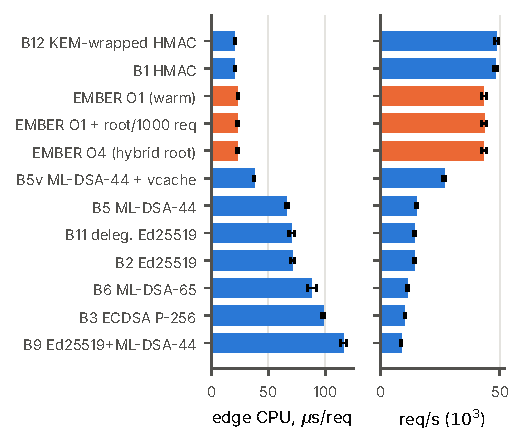
\includegraphics[width=\columnwidth]{figures/fig11_proto_capacity.pdf}
\caption{Edge capacity of the Go prototype (P1, quiet rerun, one edge core, edge utilization $\ge0.99$ in all runs; mean and 95\% $t$-CI over 5 runs). Left: edge CPU per HTTP request (primary metric). Right: requests/s.}
\label{fig:capacity}
\end{figure}

\textbf{Whole-request edge cost (P1).} Fig.~\ref{fig:capacity} shows the cost of a complete HTTP request, including Go's request parsing and response, on a single saturated edge core. Edge utilization was at least 0.99 in every one of the 60 runs. A request carrying an HMAC token (B1) costs 20.54\us{} [20.25, 20.82] of edge CPU. A warm EMBER request (O1) costs 22.91\us{} [22.49, 23.33], 1.12$\times$ HMAC, and one core serves \num{43355} req/s against \num{48340} for HMAC (0.897$\times$). Per-token ML-DSA-44 (B5) costs 66.24\us{} [65.01, 67.46], 2.89$\times$ EMBER, at \num{15040} req/s. Adding a verification cache (B5v) lowers this to 37.38\us{} (\num{26620} req/s), still 1.63$\times$ EMBER, because every request must parse and hash a 3.3~KB token. Re-verifying the root every 1000 requests (O1a, 22.92\us) or using a hybrid root (O4, 22.93\us{} [22.39, 23.47]) is indistinguishable from O1. Per-request crypto and token size, not post-quantum verification as such, determine edge cost: in Go, per-token ML-DSA-44 (66.24\us) is cheaper than Ed25519 (71.04\us), B11 (70.36\us) and ECDSA P-256 (98.04\us).

\subsection{Issuer Throughput}
Per-token ML-DSA-44 signing limits a native issuer core to $1/408.8\,\mu\text{s}\approx\num{2446}$ tokens/s. EMBER with an ML-DSA-44 root issues \num{469254} tokens/s per core [\num{319698}, \num{729692}] at $N=2^8$ and \num{1275990} [\num{1161768}, \num{1282009}] at $N=2^{14}$, 192$\times$ and 522$\times$ more (Fig.~\ref{fig:sizeN}, bottom). At large $N$ the cost is dominated by leaf hashing and base64url encoding. SLH-DSA-128s, which manages only $1/306.5\,\text{ms}\approx3.26$ tokens/s when signing per token, becomes a usable root signer: \num{49063} tokens/s at $N=2^{14}$. Its 306~ms signature, however, lies on the issuance path. In simulation it raises $D$ from 0.575~s to 0.927~s in pull mode at $\Delta=1$~s. B11 is not comparable to EMBER on issuance, contrary to our hypothesis: native Ed25519 signing (30.1\us) limits it to about \num{33000} tokens/s, so EMBER issues at least 14$\times$ faster. B12 tokens are as cheap as HMAC to issue, but every epoch requires $E$ key wraps, which take 37.6~ms at $E=500$ in our Python implementation. The Go prototype confirms the trend independently: its issuer reaches about \num{432000} tokens/s at $N=1024$, 53$\times$ its per-token ML-DSA-44 signing.

\subsection{Latency Under Load (P2)}
Over the emulated 21~ms link at 50\% of each scheme's capacity, no scheme's added median latency relative to HMAC is distinguishable from zero, except B2 ($-1.25$~ms) and B3 ($-1.39$~ms), which run at much lower absolute rates. At 80\% load, O1's median is $-3.24$~ms [$-6.82$, 0.34] relative to HMAC, while per-token ML-DSA-44 (B5) adds 11.47~ms [5.09, 17.85]. B5v's median of 80.05~ms has a CI that spans zero because individual runs collapsed. B5 and B5v are the only schemes that push 3.3~KB URLs at 9.5k and 16.4k req/s, about 260 and 450~Mbit/s of request bytes through a userspace link emulator that sustained about 624~Mbit/s in a bulk test. We therefore attribute this tail to the link emulator, not to edge CPU, but we have not verified this. All runs completed with zero errors. Load levels were set from the earlier P1 capacities.

\subsection{Dissemination and End-to-End Latency}
\label{sec:res-dissem}

\begin{figure}[t]
\centering
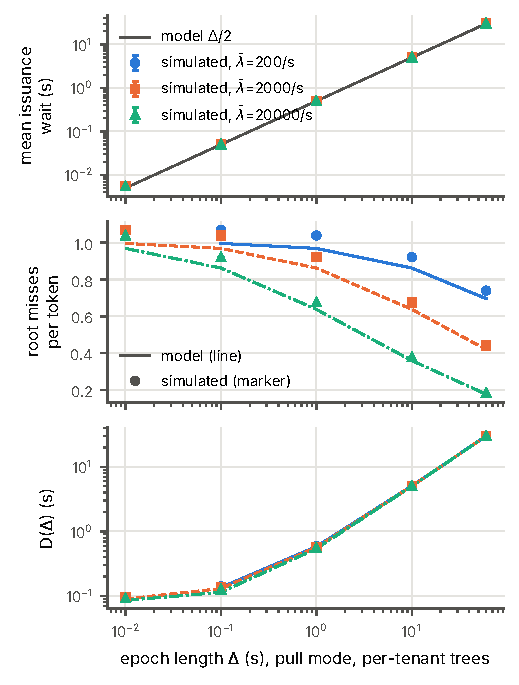
\includegraphics[width=\columnwidth]{figures/fig5_delta_tradeoff.pdf}
\caption{Pull mode, per-tenant trees (simulated, 5 seeds; model lines from Eqs.~\eqref{eq:miss}--\eqref{eq:D}). Root misses barely fall with $\Delta$ until $\lambda\Delta$ approaches $E$, so $D(\Delta)$ is minimized at the smallest $\Delta$.}
\label{fig:delta}
\end{figure}

Fig.~\ref{fig:delta} shows the trade-off that Eq.~\eqref{eq:D} predicts. Issuance wait follows $\Delta/2$. Root misses per token fall only slowly, because with $E=500$ edges and \num{1000} Zipf-distributed tenants, $\lambda_\tau\Delta\ll E$ for almost every tenant. Without re-routes the simulated misses equal Eq.~\eqref{eq:miss} to 3--4 digits. With the default mobility assumption (about 7\% of sessions switch edge once), the model under-predicts: at $\bar\lambda=2000$ and $\Delta=1$~s it gives 0.862 misses per token against 0.921 simulated.

\begin{table}[t]
\centering
\caption{Operating points (simulated; $\bar\lambda=2000$/s, $E=500$, 5 seeds, CI half-widths $<1\%$ of the mean).}
\label{tab:ops}
\footnotesize
\setlength{\tabcolsep}{3pt}
\begin{tabular}{@{}lrrrrr@{}}
\toprule
Mode & $\Delta$ (s) & misses/token & $D$ (ms) & req.\ waiting & root/served B \\
\midrule
pull & 0.01 & 1.069 & 96.2 & 0.71\% & $2.4\cdot10^{-5}$ \\
pull & 1 & 0.921 & 575.4 & -- & -- \\
pull\_staple & 0.01 & 0.073 & 11.7 & 0.049\% & $1.6\cdot10^{-6}$ \\
pull\_staple & 1 & 0.058 & -- & -- & -- \\
push & 0.01 & 0.622 & 19.8 & -- & $5.0\cdot10^{-3}$ \\
push\_rollup & 0.01 & 0.997 & -- & 0.67\% & $5.3\cdot10^{-5}$ \\
\bottomrule
\end{tabular}
\end{table}

\begin{figure*}[t]
\centering
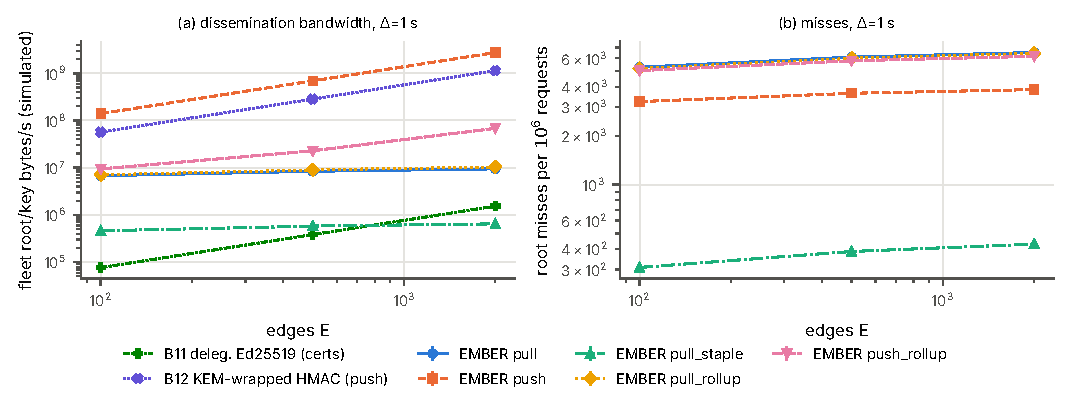
\includegraphics[width=\textwidth]{figures/fig7_dissemination.pdf}
\caption{Dissemination vs.\ fleet size ($\Delta=1$~s, $\bar\lambda=2000$/s; simulated). (a) Fleet root, key or certificate bytes/s. (b) Root misses per $10^6$ requests.}
\label{fig:dissem}
\end{figure*}

Table~\ref{tab:ops} and Fig.~\ref{fig:dissem} compare the modes. \textbf{Stapling is the decisive mode.} It reduces misses per token from 1.069 to 0.073 at $\Delta=0.01$~s, and the remaining misses come only from mid-session re-routes: 0 when no re-routes occur, 0.56 when the re-route probability is 0.005. It also cuts mean added delay $D$ from 96.2~ms to 11.7~ms and the share of requests that wait for a root from 0.71\% to 0.049\%. At $E=500$ it gives 387 misses per $10^6$ requests, against \num{6098} for pull. Root traffic is $1.6\cdot10^{-6}$ of served bytes, and fleet root bandwidth is 0.46--0.65~MB/s for $E=100$--2000. \textbf{Push} at $\Delta=0.01$~s needs 2.27~GB/s of root traffic. Even at $\Delta=1$~s it needs 140~MB/s to 2.75~GB/s for $E=100$--2000, and it still misses 0.622 per token at $\Delta=0.01$~s, because the 150~ms push delay exceeds the 120~ms between token receipt and first request. \textbf{Roll-up} did not deliver the 5$\times$ miss reduction we hypothesized. It removes only 1.4--2.2\% of misses (\num{6098}$\to$\num{6011} per $10^6$ requests at $\Delta=1$~s; 1.069$\to$1.045 misses per token at $\Delta=0.01$~s), because first requests arrive about 120~ms after issuance, before any period closes. Its value lies instead in bounding edge root state and in carrying revocation deltas (mean revocation propagation 150~s in pull modes). For comparison, B12's key-wrap push needs 57~MB/s to 1.13~GB/s and B11's certificate pulls 0.08--1.5~MB/s.

\begin{figure}[t]
\centering
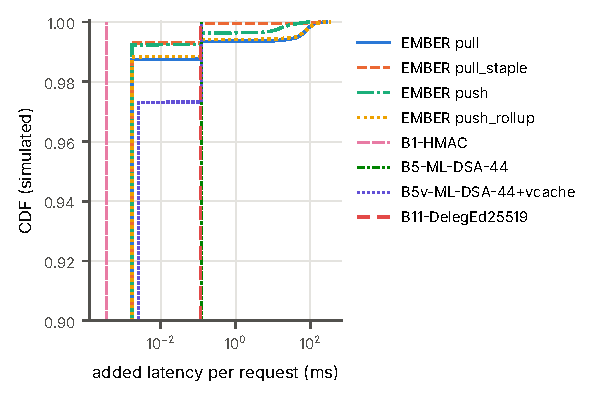
\includegraphics[width=\columnwidth]{figures/fig8_e2e_cdf.pdf}
\caption{Added latency per request (miss wait plus native verification CPU; simulated, $5\times\num{20000}$ samples per curve). Upper tail shown.}
\label{fig:e2e}
\end{figure}

Fig.~\ref{fig:e2e} shows the per-request added latency. With stapling, p99 is 0.0017~ms, 0.05\% of requests exceed 1~ms and p99.9 is 0.12~ms. Plain pull has p99 0.123~ms and p99.9 112~ms, where root-miss round trips dominate. Per-token ML-DSA-44 adds 0.122~ms to \emph{every} request, and B5v has p99 0.125~ms. Simulated edge CPU, including amortized root verification, is 1.2--1.7\us{} per request for EMBER in pull mode.

\emph{Hybrid root.} The hybrid root leaves warm per-request cost unchanged (20.27 vs.\ 19.98\us{} in Python, +1.5\%). In the Go prototype O4 and O1 differ by 0.09\% per request, with overlapping CIs (Section~\ref{sec:res-cpu}). With per-tenant trees, however, each (edge, epoch) root serves about one session, so the additional Ed25519 root verification raises \emph{simulated} mean edge CPU per request by 41.6\% (2.37 vs.\ 1.67\us). The absolute cost remains at the microsecond level, but our hypothesis of a $<1\%$ change is refuted.

\subsection{Epoch Control}
\label{sec:res-controller}

\begin{table}[t]
\centering
\caption{24-h diurnal workload, pull mode (simulated). $D$ in ms [95\% $t$-CI]. Paired: adaptive minus policy (common random numbers).}
\label{tab:controller}
\footnotesize
\setlength{\tabcolsep}{1.8pt}
\begin{tabular}{@{}lrrrr@{}}
\toprule
$\bar\lambda$ (seeds) & adaptive $D$ & best fixed $D$ & paired diff. & WC $D$ \\
\midrule
200 (10) & 96.61 & 96.61 ($\Delta$=0.01) & $-0.001$ [$-0.004$, 0.002] & 91.68 \\
2000 (10) & 96.08 & 96.08 ($\Delta$=0.01) & $+0.005$ [0.001, 0.010] & 91.68 \\
\num{20000} (5)$^\ast$ & 90.40 & 91.23 ($\Delta$=0.01) & $-0.83$ [$-0.91$, $-0.75$] & 91.45 \\
\bottomrule
\multicolumn{5}{@{}l}{\scriptsize $^\ast$1-h peak window. Best fixed $\Delta$ chosen in hindsight per rate decile.}
\end{tabular}
\end{table}

Table~\ref{tab:controller} reports hypothesis H5, which failed. The adaptive controller chose the grid floor, $\Delta=10$~ms, almost all day, and matched the best fixed $\Delta$ chosen in hindsight to within $-0.83$ to $+0.005$~ms (at most 0.9\%). This is far below the pre-registered 10~ms / 10\% threshold, so we demote the controller to a design guideline. A work-conserving close beat it by 4.93~ms and 4.41~ms at $\bar\lambda=200$ and 2000. It was 1.0~ms worse at \num{20000}, where the adaptive policy was best. Fixed $\Delta\ge3$~s violated the 2~s issuance SLO in every 5-min bin. The interior optimum predicted by Eq.~\eqref{eq:D} did not occur for any tenant at $\bar\lambda\le2000$, because misses do not fall until $\lambda_\tau\Delta\gg E$, while waiting grows linearly. With stapling, $F_{\text{miss}}$ is nearly zero, and the optimum is trivially the smallest $\Delta$ the signer sustains.

\subsection{Simulator Validation Against the Prototype}
\label{sec:res-validate}

\begin{figure*}[t]
\centering
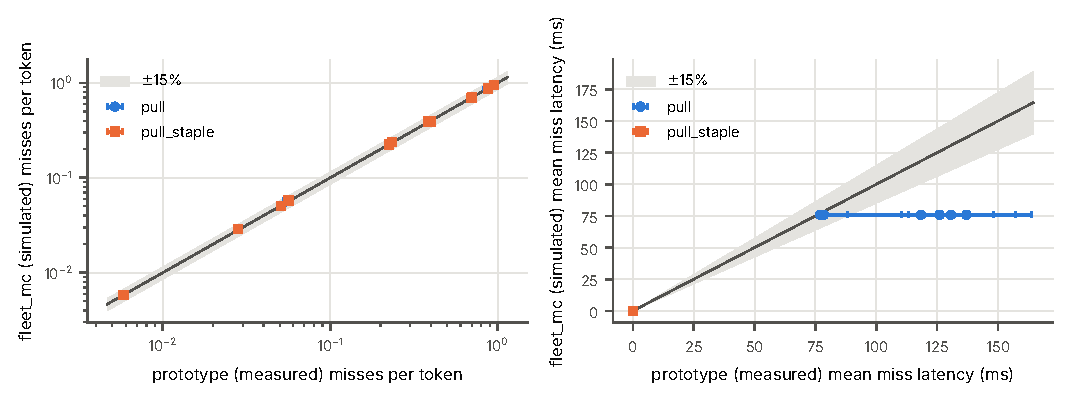
\includegraphics[width=\textwidth]{figures/fig12_proto_validation.pdf}
\caption{Simulator (fleet Monte Carlo, 50 seeds, fed measured RTTs) vs.\ prototype (P3, 5 runs, 95\% CI) on 24 configurations. Left: misses per token, 24/24 within 15\% or inside the CI. Right: mean miss latency. Pull at $\Delta\le1$~s matches; pull at $\Delta=10$~s and stapled misses do not.}
\label{fig:validate}
\end{figure*}

We ran the simulator with the prototype's P3 configuration and its measured RTT distribution, and compared it with the prototype (Fig.~\ref{fig:validate}). For \emph{misses per token} and \emph{root bytes per token}, 24 of 24 configurations pass (relative error at most 15\% or simulator inside the prototype CI). The maximum error is 4.4\% for the simulator and 14.8\% for the steady-state model, whose error at $\Delta=10$~s comes from partly filled boundary epochs in the 60~s window. For example, at $V=10$, $\Delta=1$~s and $\lambda=200$/s the prototype measures 0.05116 [0.05036, 0.05196] misses per token and the simulator predicts 0.05067. For \emph{mean miss latency}, pull at $\Delta\le1$~s passes in 8 of 8 configurations (prototype 76.9--78.5~ms, simulator 75.9~ms). The other configurations fail. Pull at $\Delta=10$~s measures 118--137~ms against 75.9~ms predicted. The four concurrent pipelines' timers are aligned, so each epoch close releases about \num{4400} tokens whose first requests reach the one-core edge within about 200~ms. First-request p50 latency is 136.8~ms at $\Delta=10$~s versus 23.6~ms at $\Delta=1$~s. The simulator has no edge-CPU or link queueing. Stapled misses measure 0.074--0.086~ms against 0.026~ms predicted, because the simulator charges only signature verification, not decoding the 3.3~KB header. That absolute gap is about 0.05~ms. We therefore scope the simulator's latency claims to non-bursty edges. Its miss and byte predictions are validated.

\subsection{Denial of Service}
\label{sec:res-dos}
We flooded one simulated edge with \num{10000} fake tokens/s. When the fake epochs are spread over all tenants, coalescing and negative caching do \emph{not} help, because keys rarely repeat: 9270--9636 root fetches/s, 4630 signature verifications/s and 0.48 of one core. Restricted to the lowest-rate tenant, coalescing reduces fetches from 7680/s to 65/s. A stapled-root flood costs \num{10000} verifications/s, 1.03 cores. A per-client limit of one staple per second (100 clients) reduces this to 100/s and 0.027 of a core. Per-client limits on fetches and staples are therefore required. Coalescing and negative caching protect only against single-tenant floods.

\subsection{Trust and Cost Summary}

\begin{table*}[t]
\centering
\caption{Trust and cost comparison. Bytes: measured token, 60-character path. Verify: native OpenSSL~3.5.4 median per request (EMBER: path, $d=16$). Dissemination: simulated fleet bytes/s for $E=500$, $\bar\lambda=2000$/s, $\Delta=1$~s.}
\label{tab:trust}
\footnotesize
\setlength{\tabcolsep}{4pt}
\begin{tabular}{@{}lllp{2.6cm}rp{2.2cm}r@{}}
\toprule
Scheme & Secret at edge & One compromised edge mints for & PQ assumption & Bytes & Verify (\textmu s) & Dissem.\ (kB/s) \\
\midrule
B1 HMAC & yes (key lifetime) & all edges, all paths of the key & unconditional & 166 & 0.30 & 0 \\
B10 multi-MAC, $k{=}3$ & yes & its own domain & unconditional & 187 & 0.30 & 0 \\
B12 KEM-wrapped HMAC & yes (epoch keys) & all edges, live epochs & unconditional (ML-KEM) & 171 & 0.30 & \num{283521} \\
B2 Ed25519 & no & none & none (Shor) & 209 & 94.6 & 0 \\
B11 delegated Ed25519 & no & none & classical security within $\vmax$ & 214 & 94.6 & 383.2 \\
B5 ML-DSA-44 & no & none & unconditional & \num{3350} & 100.9 & 0 \\
B5v + verify cache & no & none & unconditional & \num{3350} & 100.9 first, 2.19 hit & 0 \\
EMBER O1 (pull) & no & none & unconditional & 503 & 2.34 (+root per epoch) & \num{8411} \\
EMBER O1 (push) & no & none & unconditional & 503 & 2.34 & \num{689374} \\
\bottomrule
\end{tabular}
\end{table*}

Table~\ref{tab:trust} summarizes the comparison. The B5v hit cost (2.19\us) is the SHA-256 cache key over a 3.5~KB token. EMBER is not the best scheme on every metric. B11 and B12 have smaller tokens, and HMAC-based schemes have cheaper verification. Among the schemes we compared, EMBER is the only one that is at once (i) post-quantum without a time-bounded classical assumption, (ii) free of minting secrets at edges and (iii) small enough for URLs and cookies. Its costs are a root-dissemination path and tokens about 3$\times$ larger than HMAC tokens.
